\bexo

On pose

\begin{equation}
	f(x) = \sin(x) ~~,~~
	% g(x) = x^2 ~~,~~
	g(x) = \begin{cases}
			1 & si~x\leq 0\\
			-1 & sinon
		\end{cases}
\end{equation}

Tracer $h_1(x) = f(x)+g(x)$ et $h_2(x) = f(x)\times g(x)$.

\begin{center}
	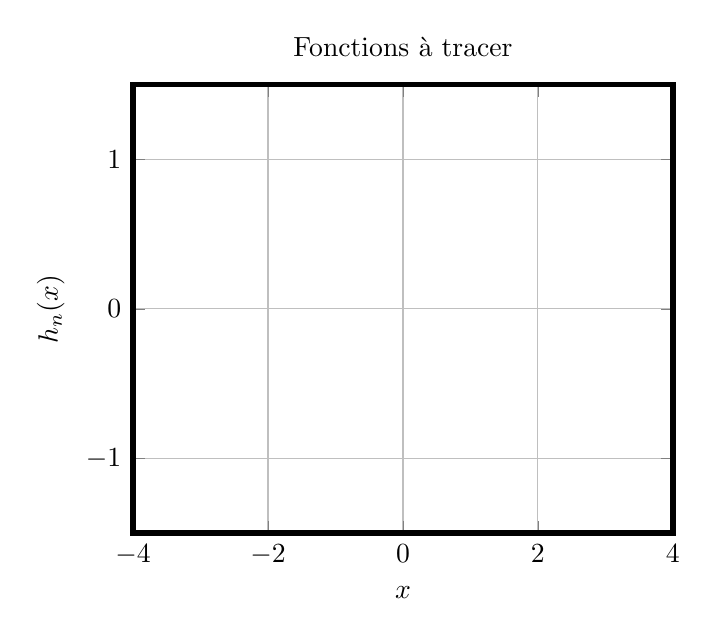
\begin{tikzpicture}
		\begin{axis}[
			line width=2pt,
			legend columns=-1,
			title=Fonctions à tracer,
			xlabel={$x$},
			ylabel={$h_n(x)$},
			xmin=-4,
			xmax=4,
			ymin=-1.5,
			ymax=1.5,
			legend to name=named,
			grid=major]
		\end{axis}
	\end{tikzpicture}
\end{center}
\eexo
\solution{\hfill\\
	Les graphes des fonctions sont:
	\begin{center}
		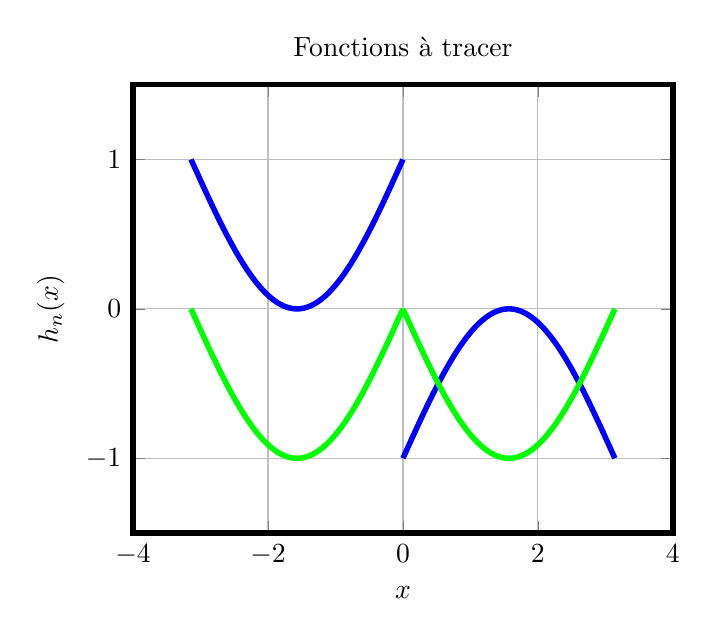
\begin{tikzpicture}
			\begin{axis}[
				line width=2pt,
				legend columns=-1,
				title=Fonctions à tracer,
				xlabel={$x$},
				ylabel={$h_n(x)$},
				xmin=-4,
				xmax=4,
				ymin=-1.5,
				ymax=1.5,
				legend entries={$h_1(x)$, $h_2(x)$},
				legend to name=named,
				grid=major]
			\addplot[blue,samples=500] expression[domain=-pi:0]{1+sin(180*x/pi)};
			\addplot[green,samples=500] expression[domain=-pi:0]{sin(180*x/pi)};

			\addplot[blue,samples=500] expression[domain=0:pi]{-1+sin(180*x/pi)};
			\addplot[green,samples=500] expression[domain=0:pi]{-sin(180*x/pi)};
			\end{axis}
		\end{tikzpicture}
		\ref{named}
	\end{center}
}

